% ----------------------------------------------------------------------
% ----------------------------------------------------------------------
\section*{Gradientenverfahren}
\subsection*{Gradient}
Der \emph{Gradient} ist ein Vektor $g$, der für jeden differenzierbaren Punkt einer Funktion $f$ definiert ist. Er deutet von diesem Punkt aus in die Richtung des \emph{steilsten Anstiegs} und gibt durch seinen Betrag $|g|$ den Steigungsgrad in diese Richtung an.

Der Gradient ist also die \emph{Verallgemeinerung der Ableitung für mehrdimensionale Funktionen}. Folglich deutet der negative Gradient $-g$ genau in die Richtung des steilsten Abstiegs.

Der Operator für einen Gradienten $\nabla$ wird als \emph{Nabla-Operator} bezeichnet. Die Schreibweise für einen Gradienten $g$ des Punktes $(x,y)$ einer zweidimensionalen Funktion $f$ lautet:
\[
	g(x,y) = \nabla f(x,y)
\]

\subsection*{Gradientenabstieg}
Alle Gradientenverfahren (engl. gradient descent) berechnen den Gradienten einer Zielfunktion, hier der Fehlerfunktion, und steigen entweder orthogonal zum Gradienten nach oben, bis ein Maximum erreicht ist oder nach unten, bis ein Minimum erreicht ist.
Hier wird versucht, durch Änderung der Gewichte den Fehler zu minimieren, indem eine Änderung aller Gewichte um einen Bruchteil des negativen Gradienten der Fehlerfunktion vorgenommen wird.
Es gilt der Zusammenhang, welcher schon im vorherigen Abschnitt bei den Fehlerfunktionen behandelt wurde:
\begin{align*}
	\Delta w &= - \eta \nabla Err(w) \\
	\Delta w_{i,\Omega} &= - \eta \frac{\partial Err(w)}{\partial w_{i,\Omega}}
\end{align*}

\begin{figure}[ht!] \centering 
	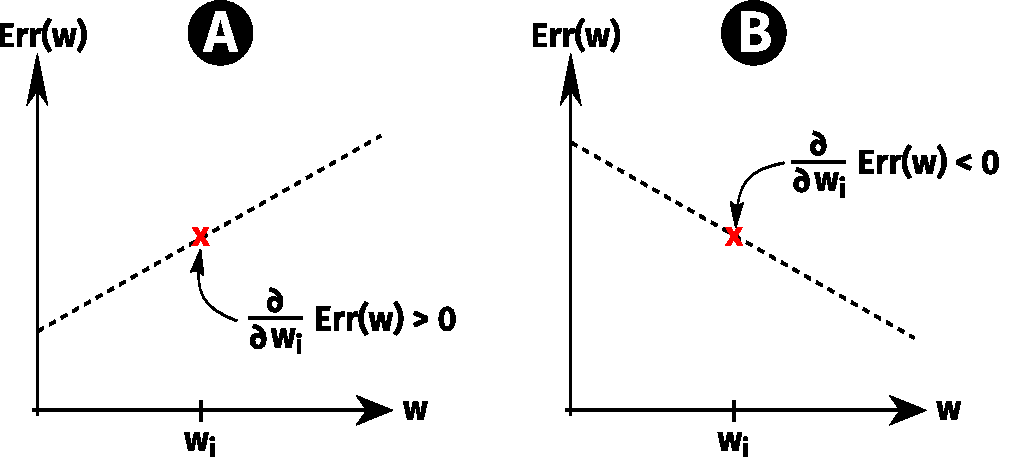
\includegraphics[width=\linewidth]{figures/ch03_gradient-decent.pdf}
	\caption{Gradientenabstieg grafisch dargestellt. Im Fall \emph{A} ist die Steigung der Fehlerfunktion beim Gewicht $w_i$ positiv, das Gewicht muss demnach verkleinert werden, damit der Fehler kleiner wird. Im Fall \emph{B} hingegen ist die Steigung bei $w_i$ negativ, das Gewicht muss dementsprechend erhöht werden, um die Kosten zu reduzieren. Dies ist der Grund für das Minuszeichen in der Gleichung.}
	\label{fig:ch03_fehlerflaeche}
\end{figure}

Auch beim Gradientenabstiegsverfahren unterscheidet man zwischen online und offline Verfahren: 
\begin{itemize}
	\item \emph{Stochastic Gradient Descent} - Die Anpassung der Gewichte findet nach jedem Trainingsbeispiel statt. Daher ist dieses Verfahren robuster gegen nicht-konvexe Fehlerfunktionen. 
	\item \emph{Batch Gradient Descent} - Hier werden die Änderungen der Gewichte über eine Epoche hinweg aufaddiert und erst anschließend auf die Gewichte angewandt.
\end{itemize}



% ----------------------------------------------------------------------
% ----------------------------------------------------------------------
\section*{Prinzip von Backpropagation}
Backpropagation ist ein \emph{Gradientenabstiegsverfahren} und die Erweiterung der Delta-Regel auf mehrere trainierbare Gewichtsschichten, weil bei mehrstufigen Netzen keine erwünschte Ausgabe als Lerneingabe (teaching input) für die Zellen \emph{innerer Ebenen} vorhanden ist.

Wenn man den Fehler eines neuronalen Netzes als Funktion der Gewichte des Netzwerks graphisch aufträgt, erhält man eine Fehlerfläche, welche sich im zweidimensionalen Fall anschaulich graphisch darstellen lässt.

\begin{figure}[ht!] \centering 
	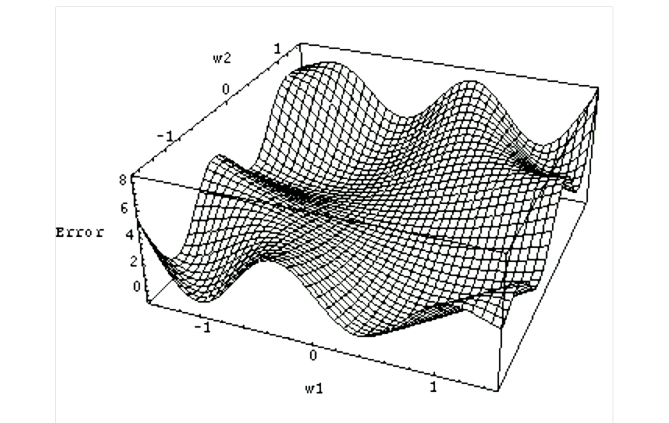
\includegraphics[width=\linewidth]{figures/ch03_fehlerflaeche.pdf}
	\caption{Fehlerfunktion $Err(w_1, w_2)$ grafisch aufgetragen.}
	\label{fig:ch03_fehlerflaeche}
\end{figure}

Abbildung \ref{fig:ch03_fehlerflaeche} zeigt die Fehlerfunktion $Err(w_1, w_2)$. Bei $n$ Gewichten gilt allgemein:
\[
	Err(\vec{w}) = Err(w_1, \ldots, w_n)
\]
Diese Fehlerfunktion gibt den Fehler an, den das Netz bei gegebenen Gewichten $w_1, \ldots, w_n$ über alle Trainingsmuster aufsummiert besitzt.

Mit einem Gradientenverfahren, d.h. der Methode des steilsten Abstiegs, wird nun versucht, möglichst schnell ein globales Minimum der Fehlerfunktion zu finden, d.h. eine Konfiguration der Gewichte, bei der die Fehlersumme über alle Trainingsmuster minimal ist.



% ----------------------------------------------------------------------
% ----------------------------------------------------------------------
\section*{Verallgemeinerung der Delta-Regel}
Zur Veranschaulichung der verallgemeinerten Delta-Regel, genannt \emph{Backpropagation of Error} oder kurz \emph{Backpropagation} dient das in Abbildung \ref{fig:ch03_fehlerflaeche} dargestellte Multi-Layer-Perzeptron (MLP).
Formal ergibt sich daraus folgender Zusammenhang:
\begin{align*}
	\Delta w_{k,h} &= \eta \cdot o_k \cdot \delta_h \\
	&\text{mit} \\
	\delta_h &=
	\begin{cases}
		f'_{act}(net_h) \cdot (t_h - y_h) 
		\quad &\text{wenn h außen} \\
		f'_{act}(net_h) \cdot \sum_{l \in L} (\delta_l \cdot w_{h,l})
		\quad &\text{wenn h innen}
	\end{cases}
\end{align*}

\begin{figure}[ht!] \centering 
	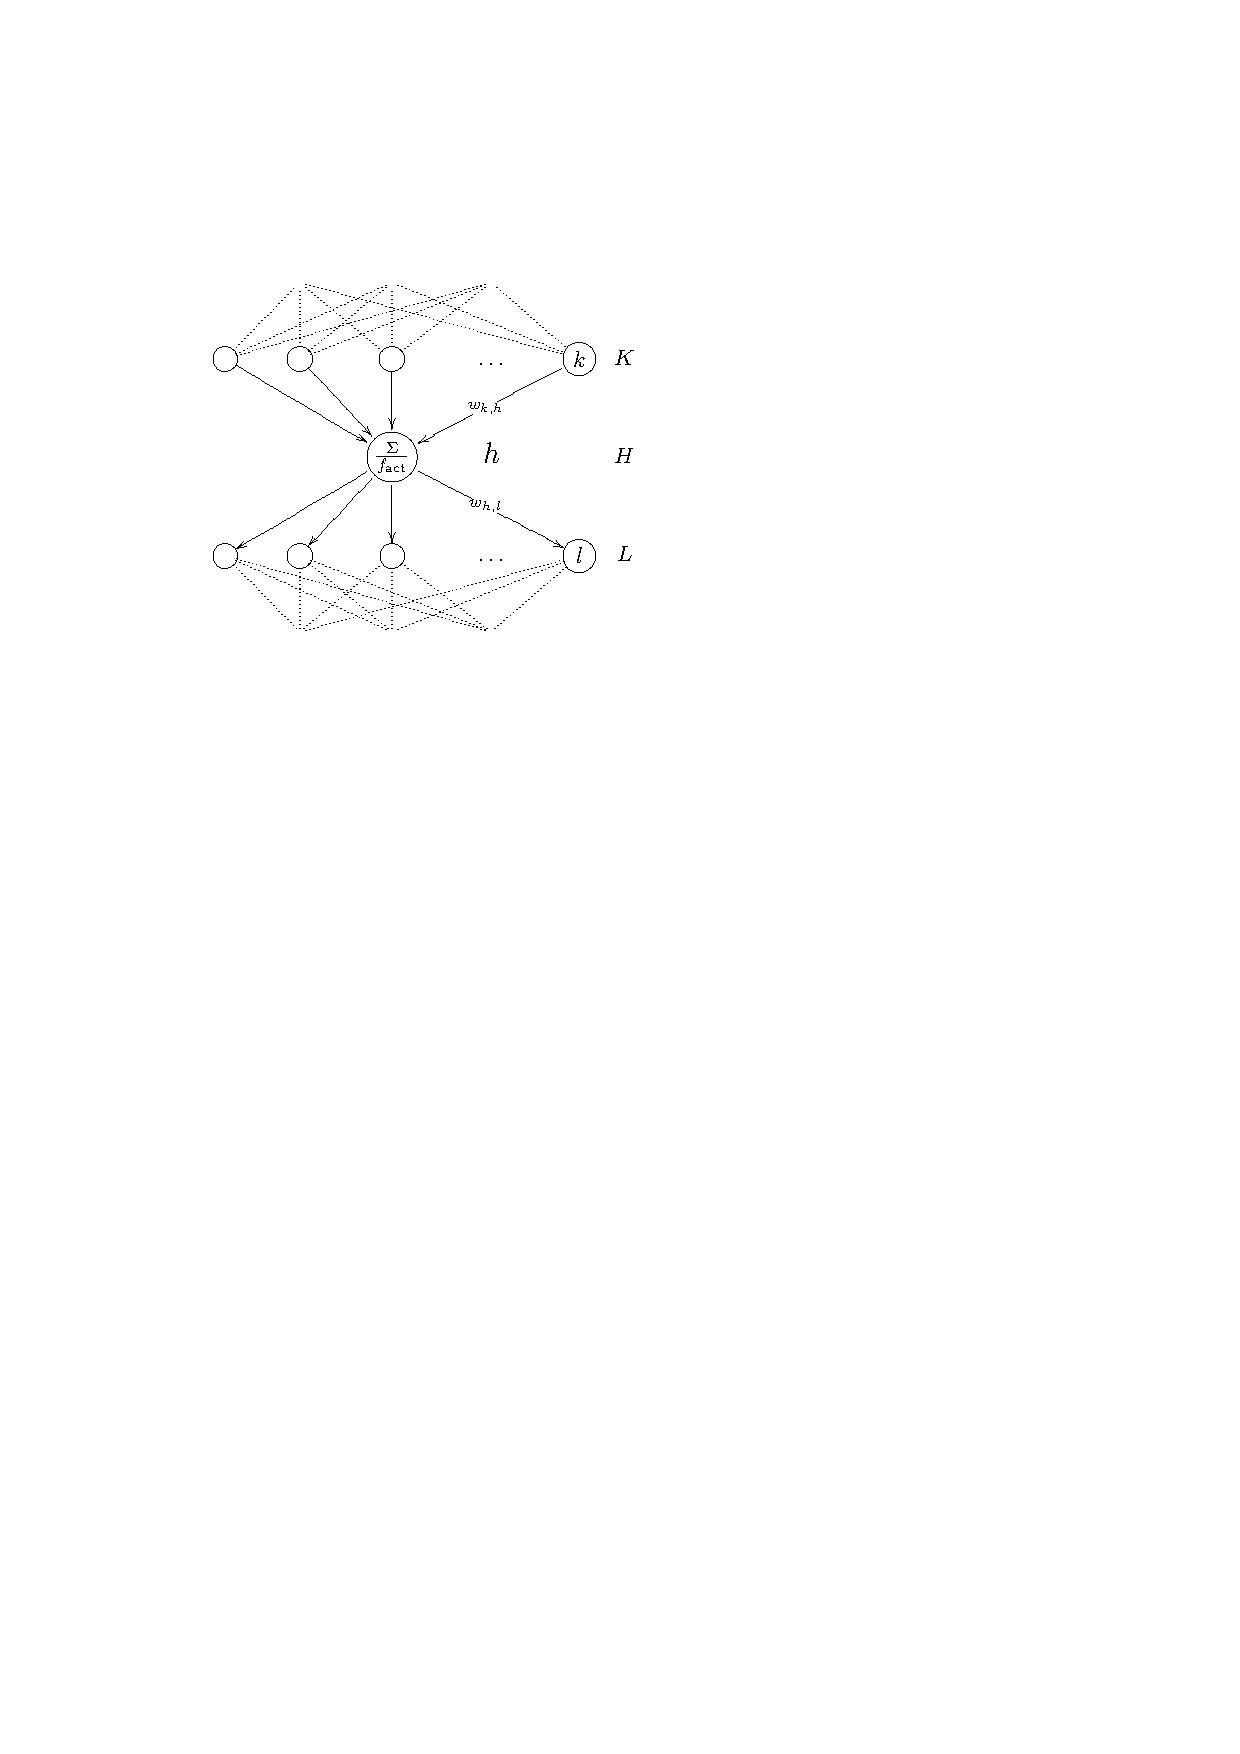
\includegraphics[width=\linewidth]{figures/ch03_mlp-backpropagation.pdf}
	\caption{Diese Abbildung zeigt die Lage des in der Formel für Backpropagation betrachteten Neurons $h$ in einer Hiddenschicht $H$. Die Vorgängerschicht ist $K$, die nachfolgende Schicht $L$. Wichtig hierbei: $L$ ist \emph{nicht} die Ausgabeschicht, sonst würde für $h$ die einfache Delta-Regel gelten.}
	\label{fig:ch03_fehlerflaeche}
\end{figure}



% ----------------------------------------------------------------------
% ----------------------------------------------------------------------
\section*{Aktivierungsfunktionen für Backpropagation}
Aus der Formel für Backpropagation geht hervor, dass die Aktivierungsfunktion semilinear, d.h. monoton und differenzierbar, sein muss. Darüber hinaus muss gelten:
\[
	f'_{act} \ne 0
\]
Werden diese Eigenschaften nicht erfüllt, so ist das Produkt für $\delta_h$ stets $0$. Eine Gewichtsänderung kann dann nicht statt finden. Deshalb eignet sich die Schrittfunktion nicht als Aktivierungsfunktion für Backpropagation.

\subsection*{Sigmoid-Aktivierungsfunktion}
Häufig wird stattdessen die Sigmoid-Aktivierungsfunktion verwendet, wie sie in Abbildung \ref{fig:ch03_sigmoid} dargestellt ist. Sie ist definiert durch:
\[
	s(x) = \frac{1}{1 + e^{-cx}} \\
\]
Für die Ableitung gilt:
\[
	\frac{d}{dx} s(x) = \frac{e^{-x}}{(1 + e^{-x})^2} = s(x)(1-s(x))
\]

\begin{figure}[ht!] \centering 
	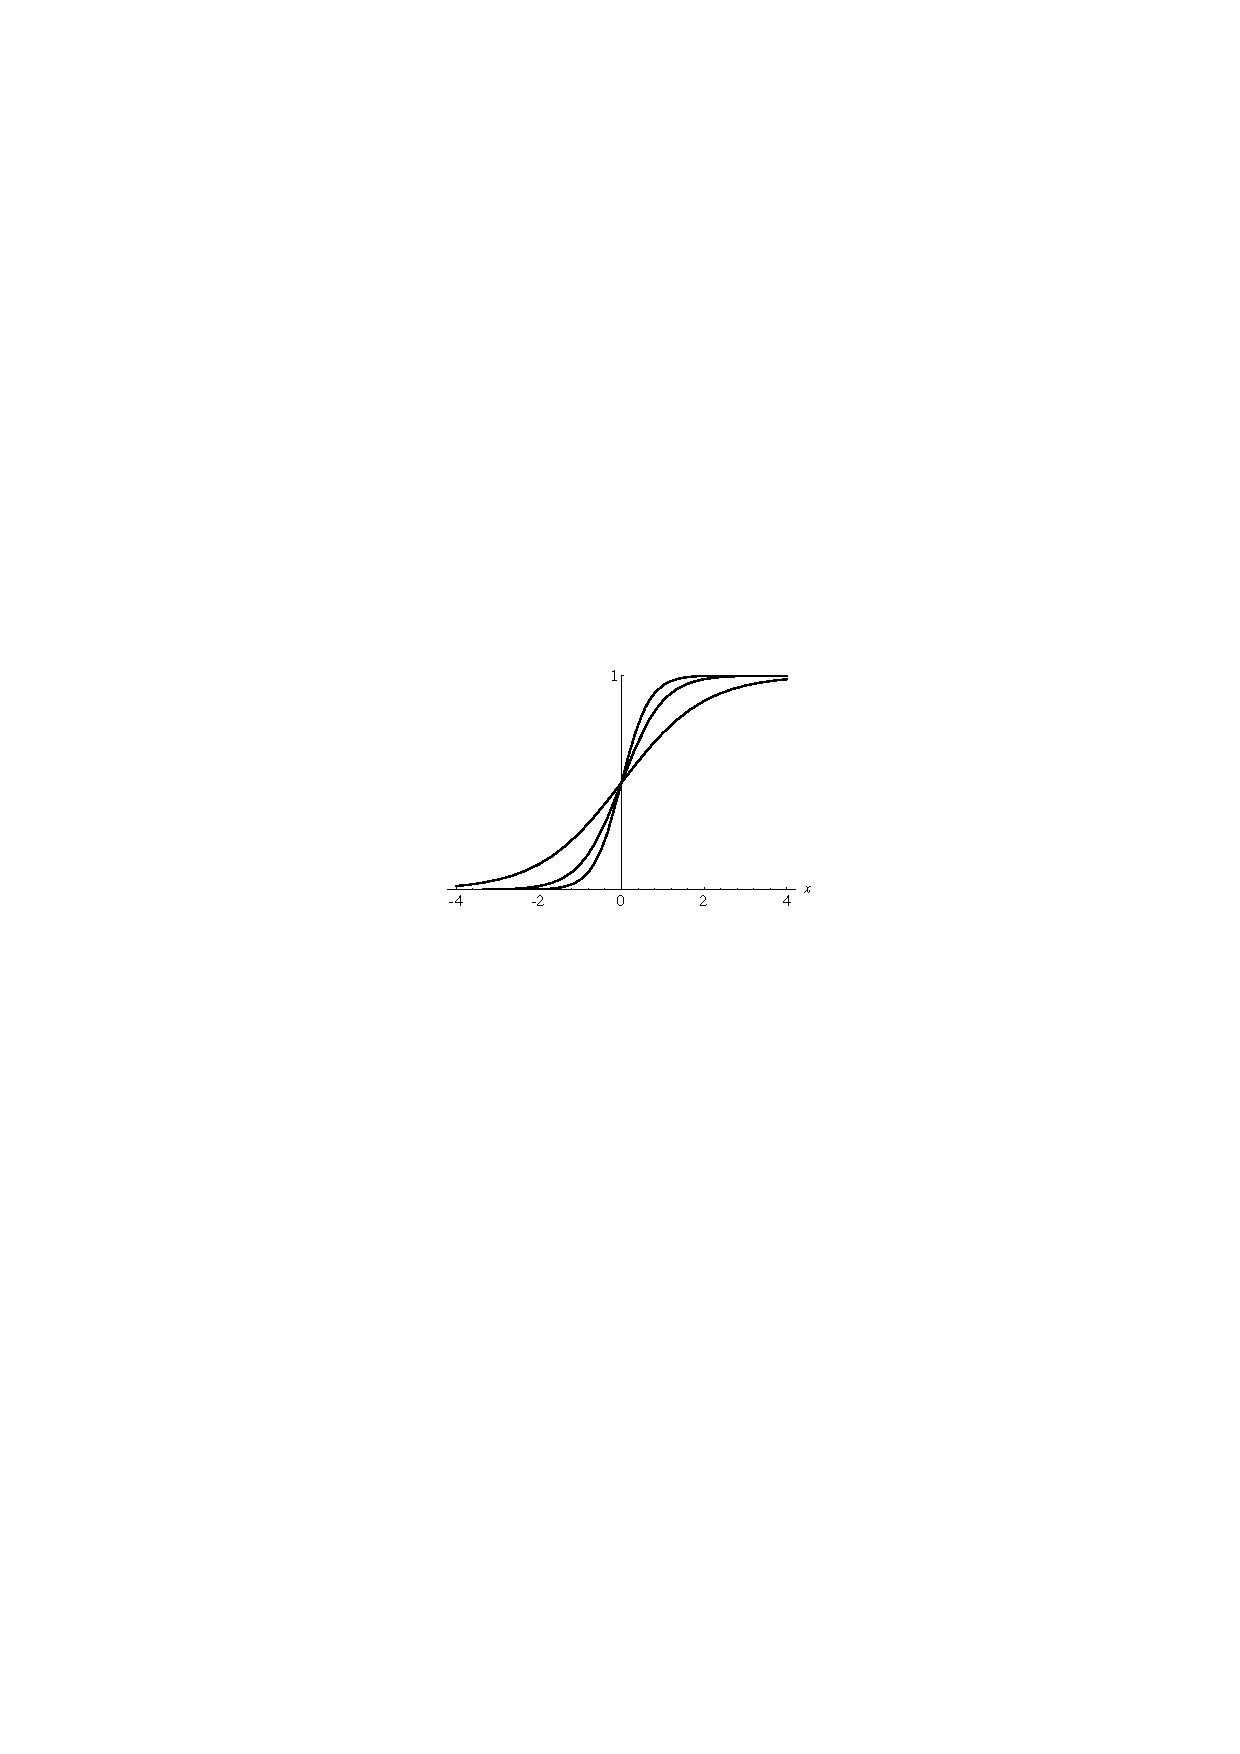
\includegraphics[width=0.7\linewidth]{figures/ch03_sigmoid.pdf}
	\caption{Verlauf der Sigmoid-Aktivierungsfunktion für $c=1$, $c=2$ und $c=3$. Je größer $c$ gewählt wird, desto steiler ist der Anstieg von $0$ auf $1$.}
	\label{fig:ch03_sigmoid}
\end{figure}



% ----------------------------------------------------------------------
% ----------------------------------------------------------------------
\section*{Algorithmus}
Im Folgenden ist der Ablauf des Backpropagation-Algorithmus aufgeführt.

\begin{itemize}
	\item zufällige Initialisierung der Gewichte
	\item Wahl eines Eingabemusters $x \in X$

	\begin{itemize}
		\item \emph{Forward propagation}: \\
			Berechnung der Netzausgabe $o_x$
		\item \emph{Backward propagation}: \\
			Fehlerrückführung durch das Netz und Berechnung des Fehleranteils je Gewicht: \\
			$\quad \frac{\partial Err(W)}{\partial w_{k,h}}
				(= - \delta_h \cdot o_k) $

		\begin{itemize}
			\item Für Ausgabeneuronen: \\
				$\delta_h = 
				\underbrace{(o_{x,h}(1-o_{x,h})}_{f'_{act}(net_{x,h})} 
				\cdot (t_{x,h}-y_{x,h})$ 
			\item Für versteckte Neuronen: \\
				$\delta_h = 
				\underbrace{(o_{x,h}(1-o_{x,h})}_{f'_{act}(net_{x,h})} 
				\sum_{l \in L} \delta_l \cdot w_{h,l}$ 
		\end{itemize}

		\item Anpassen der Gewichte: $w_{k,h} \leftarrow w_{k,h} + \eta o_k \delta_h$ 
		\item Solange wiederholen, bis Ergebnis (zu einem lokalen Minimum) konvergiert.
	\end{itemize}

\end{itemize}


% ----------------------------------------------------------------------
% ----------------------------------------------------------------------
\section*{Probleme}
Wie jedes Gradientenverfahren besitzt auch Backpropagation eine Reihe von Problemen, die dadurch entstehen, dass es ein lokales Verfahren ist, welches keine Information über die Fehlerfläche insgesamt hat, sondern nur aus der Kenntnis der lokalen Umgebung (des Gradienten bzw. bei Erweiterungen des Verfahrens zusätzlich einiger vorher besuchter Stellen der Fehlerfläche) ein Minimum suchen muss.

\begin{figure}[ht!] \centering 
	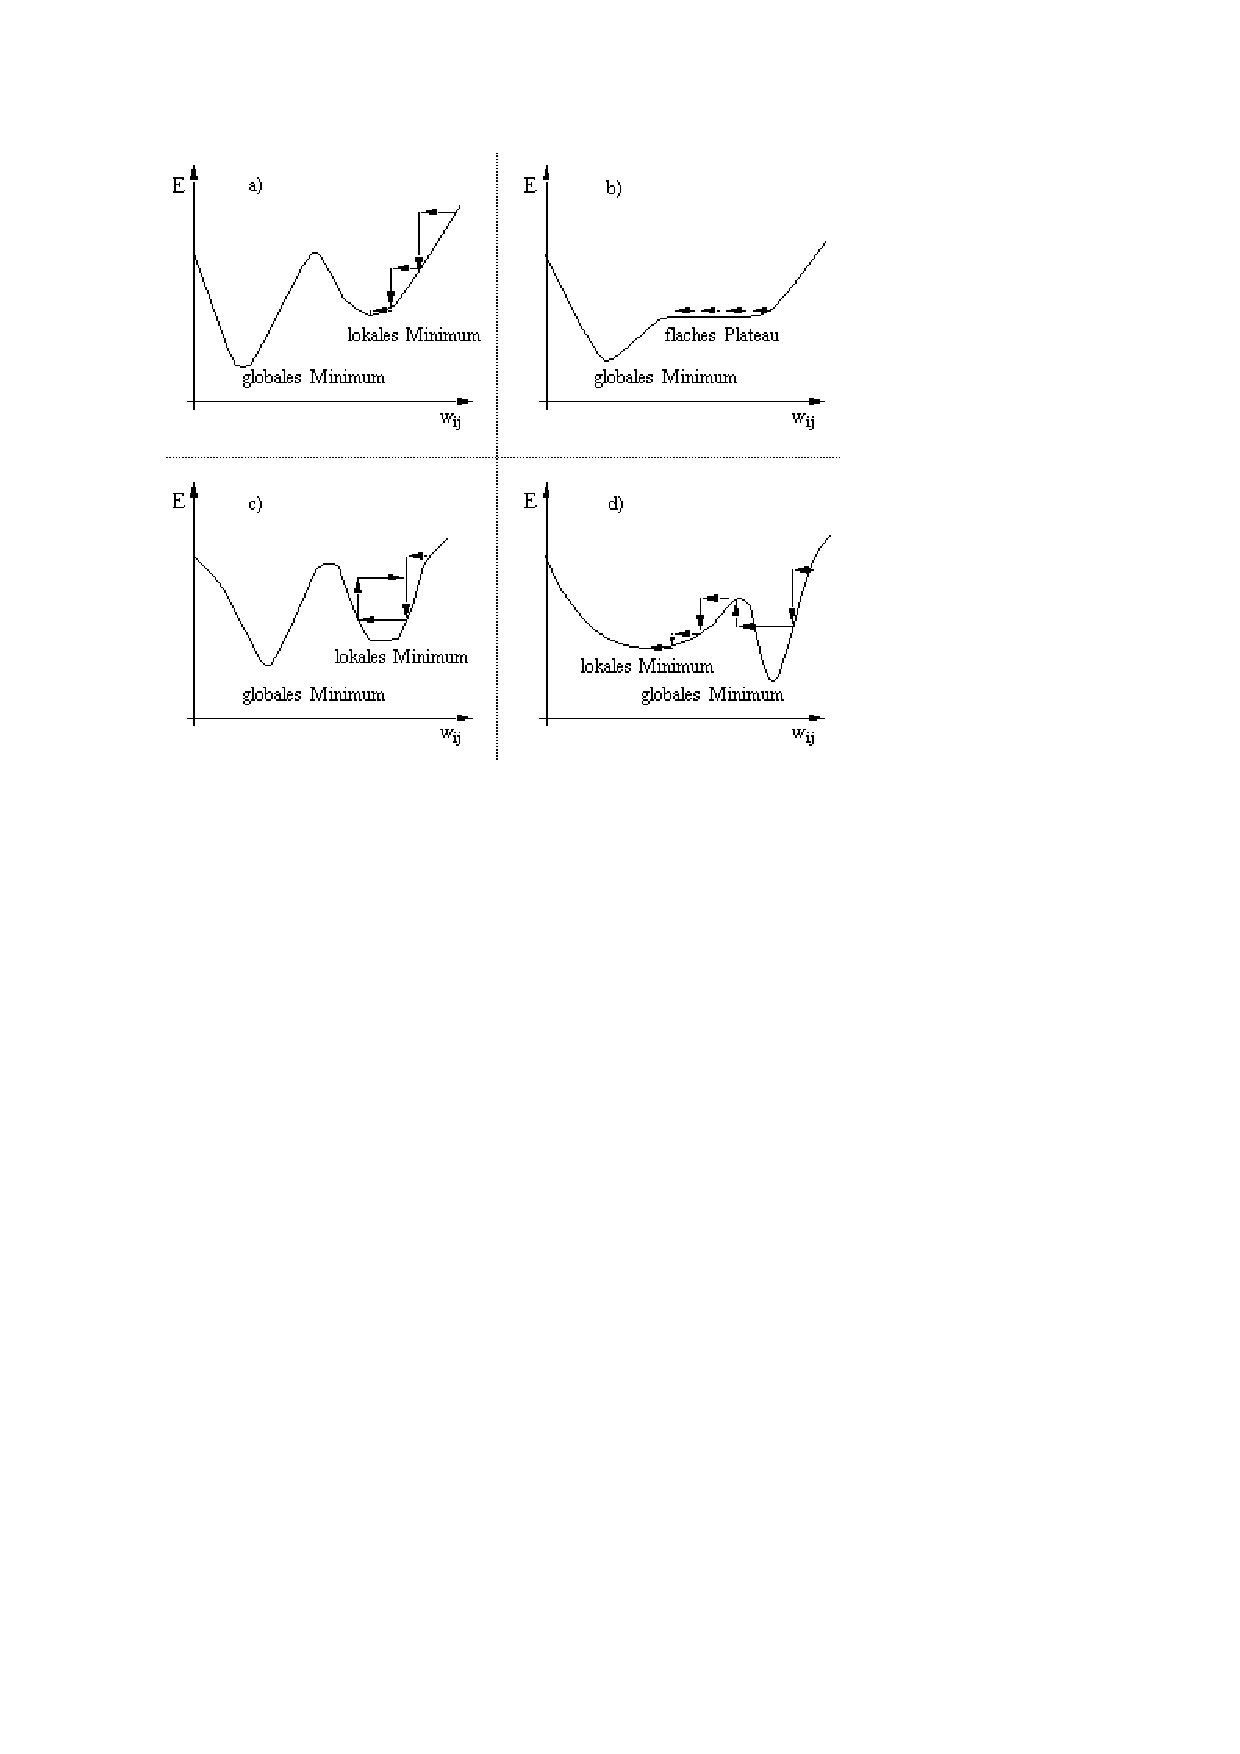
\includegraphics[width=\linewidth]{figures/ch03_fehler-gradientenverfahren.pdf}
	\caption{Problemfälle von Gradientenverfahren: a) lokales Minimum einer Fehlerfläche, b) Fehlerfläche mit Plateau, c) Oszillationen in steilen Schluchten der Fehlerfläche, d) Verlassen guter Minima}
	\label{fig:ch03_sigmoid}
\end{figure}

\subsection*{Lokale Minima der Fehlerfläche}
Gradientenverfahren haben alle das Problem, dass sie in einem lokalen Minimum der Fehlerfläche hängenbleiben können.
Das Problem neuronaler Netze ist, dass die Fehlerfläche mit wachsender Dimension des Netzes (mit wachsender Zahl von Verbindungen) immer stärker zerklüftet wird und daher die Wahrscheinlichkeit, in einem lokalen statt dem globalen Minimum zu landen, immer größer wird.

Zur Lösung solcher Probleme gibt es wenig allgemeingültigen Verfahren, weil sie stark von der Anwendung abhängen.
Die Erfahrung in der Praxis hat jedoch gezeigt, dass Backpropagation bei genügend kleiner Lernrate $\eta$ in sehr vielen Anwendungen ein Minimum findet, das gut genug am globalen Minimum liegt.

\subsection*{Flache Plateaus}
Flache Plateaus der Fehlerfläche sind ein weiteres Problem von Gradientenverfahren. Da die Größe der Gewichtsänderung von dem Betrag des Gradienten abhängig ist, stagniert Backpropagation auf flachen Plateaus, d.h. das Lernverfahren braucht extrem viele Iterationsschritte. 
Handelt es sich um ein vollständig flaches Plateau, ist der Gradient gleich dem Nullvektor und eine Gewichtsänderung findet gar nicht mehr statt.
Einen solchen Stillstand kann man dann nur schwer von dem in einem lokalen oder globalen Minimum unterscheiden, weil auch dort der Gradient ebenfalls der Nullvektor ist.

Für dieses Problem gibt es mit dem \emph{Momentum-Term}, einer Variante von Backpropagation, ein einfaches Verfahren, welches hilft diese Plateaus zu überwinden.

\subsection*{Oszillationen in steilen Schluchten}
In steilen Schluchten der Fehlerfläche kann das Lernverfahren oszillieren. Dies geschieht, wenn der Gradient am Rande einer Schlucht so groß ist, dass durch die Gewichtsänderung ein Sprung auf die gegenüberliegende Seite der Schlucht erfolgt. Ist die Schlucht dort genauso steil, bewirkt dies (da der Gradient jetzt in die andere Richtung zeigt) einen Sprung zurück auf die erste Seite.

Auch hier hilft der Momentum-Term.

\subsection*{Verlassen guter Minima}
Es ist möglich, in der Praxis aber sehr selten, dass Backpropagation aus einem guten Minimum herausspringt, weil der Betrag des Gradienten innerhalb eines sehr engen Tals der Fehlerfläche so groß ist, dass die Gewichtsänderung in ein suboptimales Minimum führt.

Gerade die Verwendung des Momentum-Terms oder die Erhöhung der Lernrate führen zu solchen Problemen.

\subsection*{Wahl der Lernrate}
Die Wahl der Lernrate $\eta$ (Schrittweite) ist entscheidend für das Verhalten des Backpropagation-Algorithmus. Zu große Werte von $\eta$ bewirken starke Sprünge auf der Fehlerfläche und bringen das Risiko mit sich, dass Backpropagation enge Täler nicht findet bzw. dass es aus ihnen wieder herausspringt oder ins Oszillieren gerät.
Zu kleine Werte von $\eta$ bringen einen großen, oft praktisch nicht akzeptierbaren Zeitaufwand für das Training mit sich.

Die Wahl von $\eta$ hängt vom Problem, den Trainingsdaten, sowie der Größe und Topologie des Netzes ab und ist nicht pauschal zu beantworten. Es gibt Verfahren zur Anpassung der Lernrate, welche in einem eigenen Abschnitt erläutert werden.



% ----------------------------------------------------------------------
% ----------------------------------------------------------------------
\section*{Modifikationen von Backpropagation}
\subsection*{Momentum-Term}
Backpropagation mit Momentum-Term (auch konjugierter Gradientenabstieg (engl. conjugate gradient descent)) wurde von Rumelhart, Hinton und Williams beschrieben.
Es ist eine einfache und häufig benutzte Methode zur Vermeidung der Probleme von Backpropagation auf flachen Plateaus und in steilen Schluchten der Fehlerfunktion. 

Die Idee dahinter ist das Einbeziehen der vorangegangenen Gewichtsänderung. Dies führt zu einer \emph{Beschleunigung} (Erhöhung der Gewichtsänderung $\Delta w_{i,j}$) in weiten Plateaus und zu einem \emph{Abbremsen} in stark zerklüfteten Fehlerflächen.

Für die Gewichtsänderung gilt dann:
\[
	\Delta w_{i,j} (t+1) = \eta \cdot o_i \cdot \delta_j + 
		\alpha w_{i,j}(t)
\]

\subsection*{Flat-Spot Elimination}
Ein bekanntes Problem der Backpropagation-Formel ist die Tatsache, dass Neuronen, die im Sättigungsbereich der sigmoiden Aktivierungsfunktion operieren (0 oder 1 bei der logistischen Aktivierungsfunktion), sich nur schwer wieder daraus entfernen, weil ihre Gewichte sich nur um einen minimalen Bruchteil ändern können.

Die Ableitung der Sigmoid-Funktion ist für Neuronen, die stark "`an"' oder "`aus"' sind, d.h. Werte um 0 oder 1 annehmen, nahezu Null. Diese Bereiche, in dem die Ableitung der Aktivierungsfunktion fast Null ist, werden daher \emph{flat spots} genannt (siehe Abbildung \ref{fig:ch03_saettigung-sigmoid-ableitung}.\footnote{Selbst im besten Fall, wenn die Netzeingabe um den Schwellenwert liegt, liefert die Ableitung der Aktivierungsfunktion einen gedämpften Faktor von $0,25$.}

\begin{figure}[ht!] \centering 
	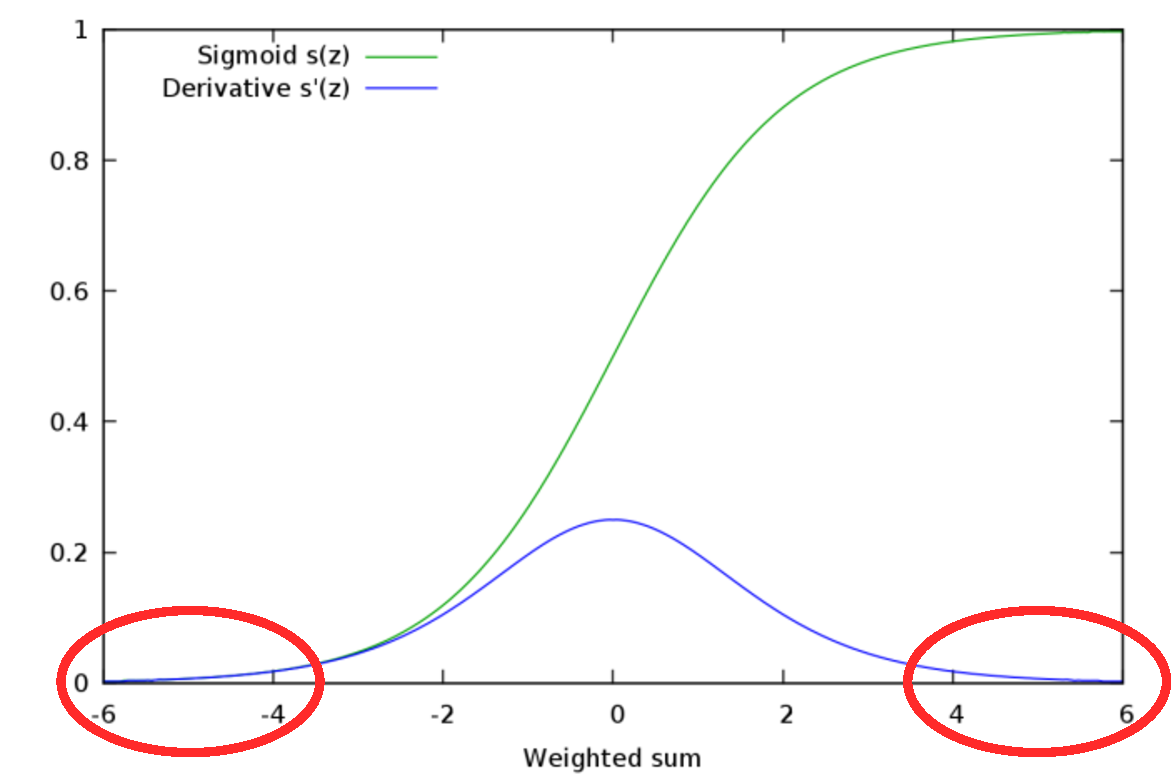
\includegraphics[width=\linewidth]{figures/ch03_saettigung-sigmoid-ableitung.pdf}
	\caption{Ableitung der Sigmoid-Funktion mit Sättigungsbereichen / \emph{flat spots} (gekennzeichnet durch Kreise).}
	\label{fig:ch03_saettigung-sigmoid-ableitung}
\end{figure}

Ein einfache Methode, dieses Problem zu beheben, ist die Anpassung der Ableitung, sodass sie nicht Null wird. Dies ist beispielsweise durch Addition einer Konstanten $0.1$ für alle Werte möglich.
Damit verläuft die Ableitung anstelle von $0$ bis $0.25$ und zurück auf $0$ jetzt von $0.1$ bis $0.35$ und zurück auf $0.1$.
In der Literatur wird diese Variante auch als \emph{modified sigmoid-prime function} bezeichnet.


\subsection*{Manhattan-Training}
Die sogenannte Manhattan-Training-Modifikation von Backpropagation geht auf Bart Sutton zurück. Dabei wird die Backpropagation-Regel durch die Regel
\[
	\Delta w_{i,j} = \eta \cdot o_i \cdot sgn( \delta_j)
\]
ersetzt, wobei die Berechnung der Fehlersignale wie bei der verallgemeinerten Delta-Regel erfolgt. Bei dieser Regel spielen nicht mehr die Beträge der Fehlersignale eine Rolle, sondern nur noch ihr \emph{Vorzeichen}. Dadurch werden die \emph{Schritte auf der Fehlerfläche quasi-normiert}, was den Problemen zu kleiner Gradienten bei flachen Plateaus und zu großer Gradienten in steilen Tälern entgegenwirkt.

Diese Quasi-Normierung ist wesentlich weniger rechenzeitaufwendig als eine richtige Normierung des Gradienten $\nabla E$ auf eine feste Länge und daher dieser meist vorzuziehen.


\subsection*{SuperSAB}
Bei SuperSAB hat jedes Gewicht eine eigene Lernrate / Schrittweite $\eta_{i,j}(t)$. Diese wird im Verlauf des Trainings kontinuierlich der Fehlerfläche angepasst. Dabei wird $\eta_{i,j}$ vergrößert, wenn die partielle Ableitung $\frac{\partial Err_p}{\partial w_{i,j}}$ für mehrere Zeitschritte das gleiche Vorzeichen hat und verkleinert, wenn sich das Vorzeichen ändert.

Für die Anpassung wird das Produkt aus der aktuellen Lernrate $\eta_{i,j}(t)$, sowie einer der Konstanten $\eta^-$ (meist $0.5$) oder $\eta^+$ (meist $1.05$) verwendet:
\begin{align*}
	\eta_{i,j}(t+1) = 
	\begin{cases}
		\eta_{i,j}(t) \cdot \eta^- &\text{falls }
			\frac{\partial E}{\partial w_{i,j}}(t) \cdot
			\frac{\partial E}{\partial w_{i,j}}(t+1) < 0 \\
		\eta_{i,j}(t) \cdot \eta^+ &\text{falls }
			\frac{\partial E}{\partial w_{i,j}}(t) \cdot
			\frac{\partial E}{\partial w_{i,j}}(t+1) > 0 \\
		\eta_{i,j}(t) &\text{sonst}
	\end{cases}
\end{align*}


\subsection*{Quickprop}
Mit dem Quickprop-Algorithmus soll eine schnelleres Training eines MLP erreicht werden. Er macht zwei "`riskante"' Annahmen:
\begin{enumerate}
	\item Die Fehlerkurve $Err(w)$ hat die Form einer Parabel
	\item Die Parabeln für jedes Gewicht $w_{h,l}$ sind unabhängig von einander.
\end{enumerate}
Diese Annahmen sind nicht richtig. Durch das iterative Einstellen der Gewichte werden die gemachten Fehler jedoch aufgehoben.

Der Algorithmus wird manchmal der Gruppe Lernverfahren zweiter Ordnung zugerechnet, da über eine \emph{quadratische} Approximation aus dem vorhergehenden Gradientenschritt $S(t-1)$ und dem aktuellen Gradienten $S(t)$ auf das Minimum der Fehlerfunktion (Scheitelpunkt der Parabel) geschlossen wird (siehe Abbildung \ref{fig:ch03_quickprop}).

Aus Abbildung \ref{fig:ch03_quickprop} geht hervor, dass die Gewichtsänderung $\Delta w_{ij}(t)$ gesucht ist, um das neue Gewicht zum Zeitpunkt $t+1$ zu bestimmen (Gewicht am Scheitelpunkt der Parabel). Aus den Ähnlichkeiten der schraffiert hervorgehobenen Dreiecke folgt dieser Zusammenhang:
\[
	\frac{\Delta w_{i,j}(t)}{\Delta w_{i,j}(t-1)} = 
		\frac{S(t)}{S(t-1) - S(t)}
\]
Daraus ergibt sich für die Gewichtsänderung $\Delta w_{i,j}(t)$ und damit für den Quickprop-Algorithmus diese Gleichung:
\[
	\Delta w_{i,j}(t) = 
		\frac{S(t)}{S(t-1) - S(t)} \cdot \Delta w_{i,j}(t-1)
\]

\begin{figure}[ht!] \centering 
	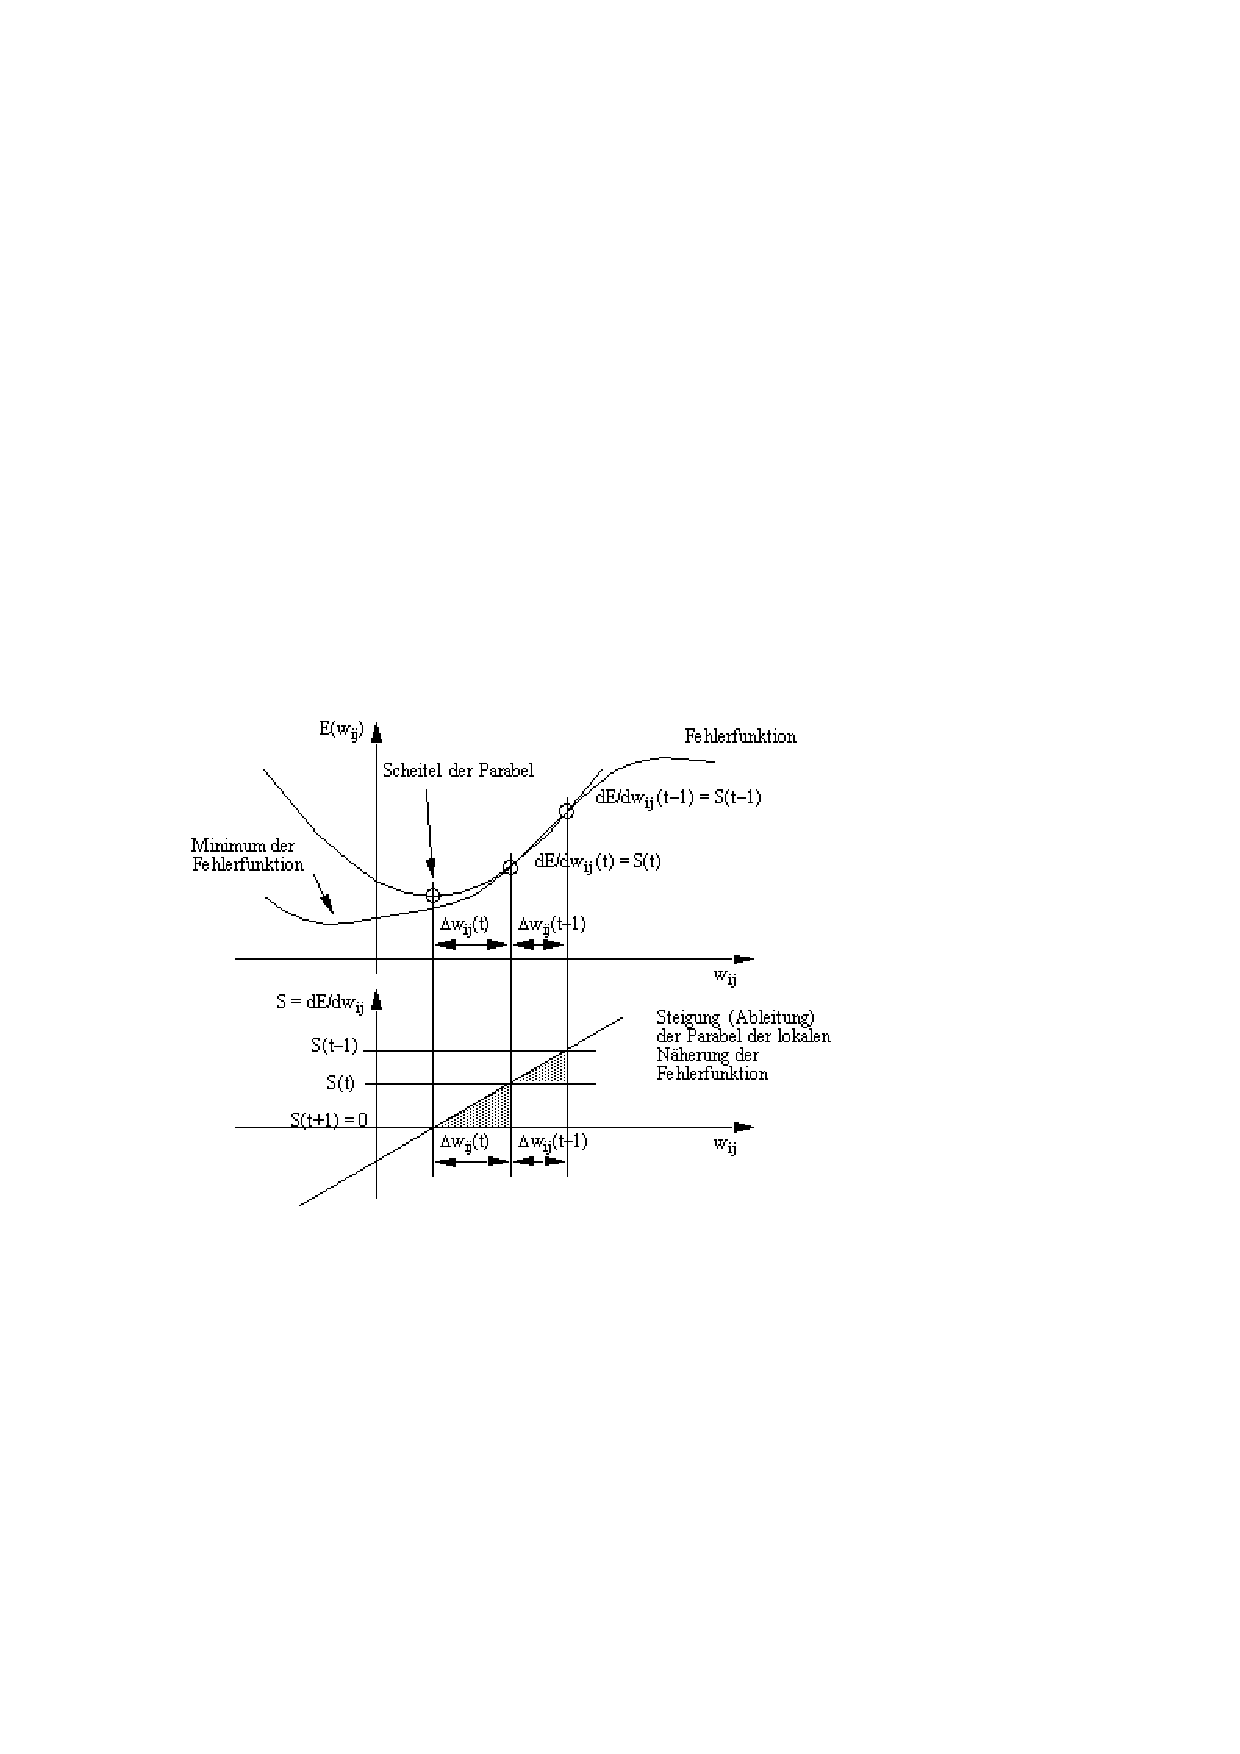
\includegraphics[width=\linewidth]{figures/ch03_quickprop.pdf}
	\caption{Idee des Quickprop-Algorithmus: Bestimmung des Scheitelpunktes der angelegten Parabel anhand der Steigung zweier verschiedener Punkte und deren Abstand. Die Abbildung zeigt oben die Fehlerkurve mit angenäherter Parabel, sowie die beiden Punkte zum Zeitpunkt $t-1$ und $t$. Unten ist die Steigung der Parabel als Gerade durch die beiden Steigungswerte $S(t-1)$ und $S(t)$ aufgetragen. Die Nullstelle gibt das Gewicht für den (angenäherten) minimalen Fehler (Scheitelpunkt der Parabel im oberen Diagramm) an.}
	\label{fig:ch03_quickprop}
\end{figure}



Der Quickprop-Algorithmus funktioniert sehr gut für hochgradig nichtlineare Probleme wie z.B. XOR. Ein beispielhaftes Trainingsverhalten ist in Abbildung \ref{fig:ch03_quickprop-training} aufgeführt.

\begin{figure}[ht!] \centering 
	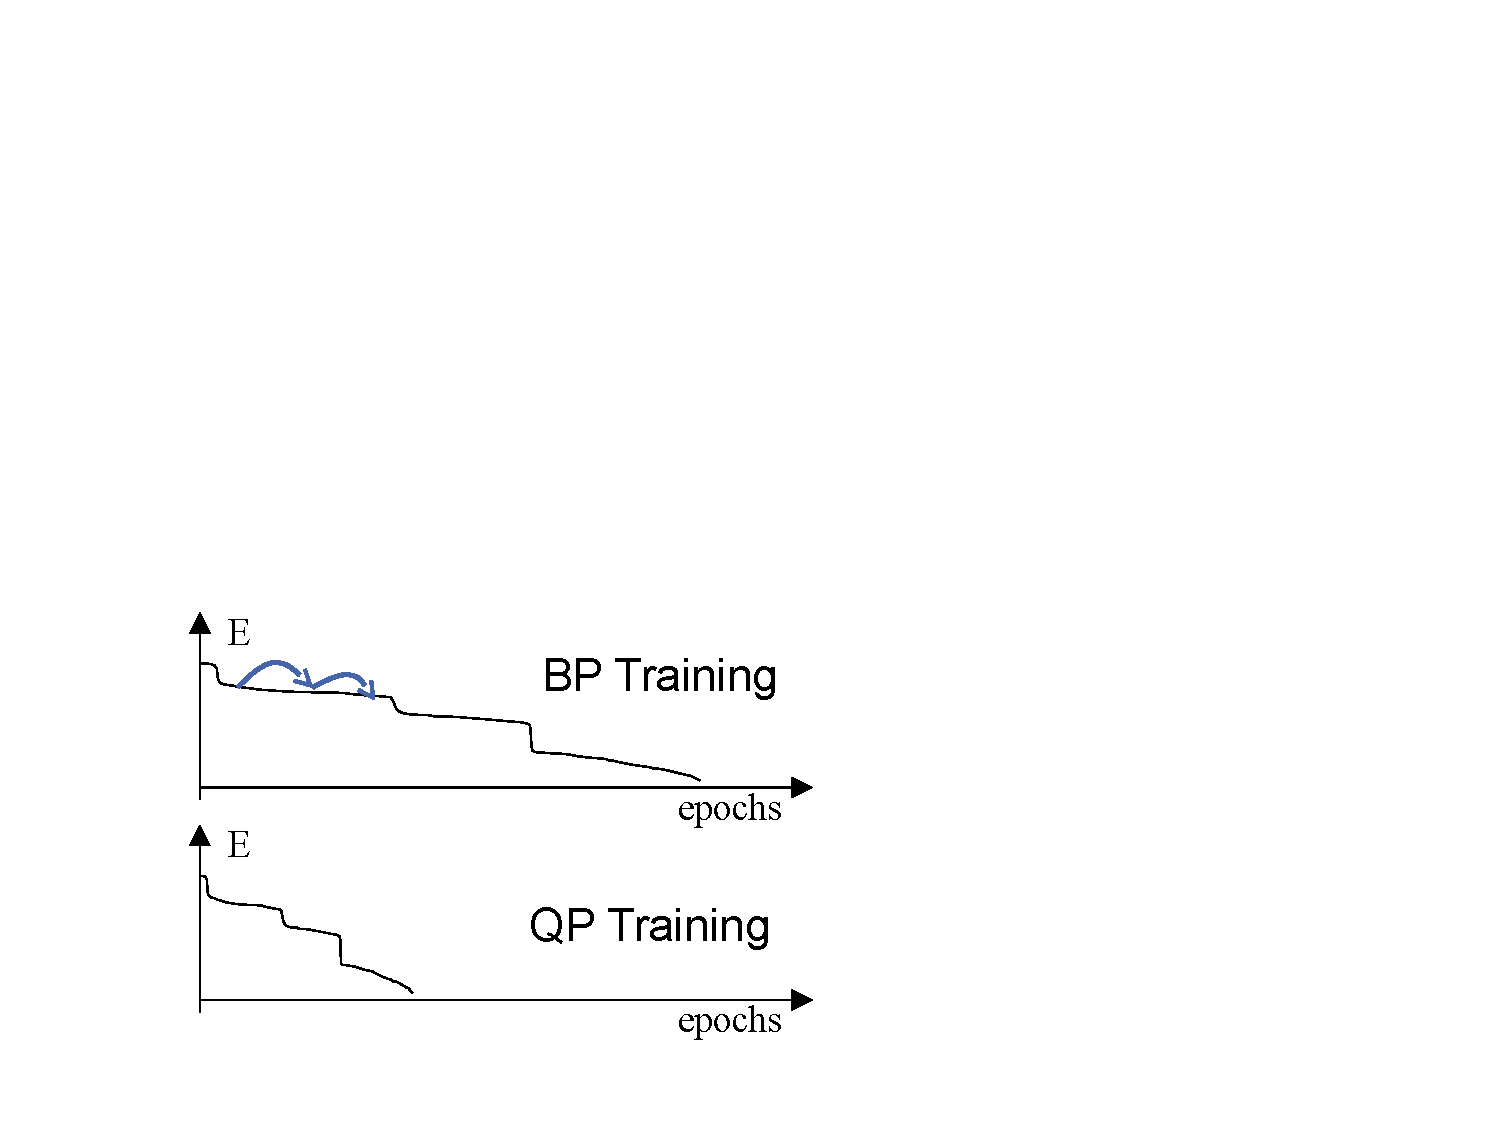
\includegraphics[width=0.7\linewidth]{figures/ch03_quickprop-training.pdf}
	\caption{Trainingsverhalten von Backpropagation (oben) und Backpropagation mit Quickprop (unten) bei hochgradig nichtlinearen Problemen.}
	\label{fig:ch03_quickprop-training}
\end{figure}

\subsection*{Rprop}
Rprop (resilient propagation) ist ein Lernverfahren, das Ideen des Manhattan-Trainings, von SuperSAB und von Quickprop kombiniert: Um die Gewichte zu aktualisieren wird nur die Lernrate $\eta$ und das Vorzeichen der partiellen Ableitung $\frac{\partial E}{\partial w_{i,j}}$ verwendet.

Dieses Vorgehen beschleunigt den Lernvorgang insbesondere in flachen Ebenen der Fehlerfunktion und nahe von lokalen Minima. Um eine zu starke Be- bzw. Entschleunigung zu verhindern existieren Minimal- und Maximalwerte ($\eta_{min}$ und $\eta_{max}$) für die Lernrate.

Wie beim Manhattan-Training werden die Gewichte nicht nach dem Gradienten der Fehlerfunktion, sondern \emph{nur nach dem Vorzeichen dieses Gradienten} geändert.
Für die Gewichts"-änderung bei Rprop gilt demnach:
\begin{align*}
	\text{es sei } g &= \frac{\partial Err(W)}{\partial w_{i,j}}\\\\
	\Delta w_{i,j} (t) &=
	\begin{cases}
		-\eta_{i,j} (t) &\text{wenn } g(t) > 0 \\
		+\eta_{i,j} (t) &\text{wenn } g(t) < 0 \\
		0 &\text{sonst} 
	\end{cases}
\end{align*}

Wie bei SuperSAB und bei Quickprop werden die Steigungen der Fehlerfunktion des aktuellen und vorherigen Zeitpunkts verwendet.
Ähnlich wie bei SuperSAB besitzt jedes Gewicht einen eigenen Parameter für die Änderung der Schrittweite.
Für die Anpassung der Lernrate $\eta_{i,j}$ wird der aktuelle Gradient $g(t)$ und der vorherige Gradient $g(t-1)$ betrachtet. Wieder ist das Vorzeichen entscheidend: Es kann über die beiden Zeitschritte gleich bleiben oder wechseln.

Wechselt das Vorzeichen von $g(t-1)$ zu $g(t)$, wurde ein lokales Minimum übersprungen, die Gewichtsänderung war zu groß.
Folglich muss die Lernrate $\eta_{i,j}(t)$ im Vergleich zu $\eta_{i,j}(t-1)$ \emph{verkleinert} werden. Dies geschieht (analog zu SuperSAB) durch Multiplikation des alten Wertes $\eta_{i,j}(t-1)$ mit der Konstanten $\eta^-$.

Bleibt das Vorzeichen jedoch gleich, kann eine (behutsame) Vergrößerung durch Multiplikation von $\eta_{i,j}(t-1)$ mit der Konstanten $\eta^+$ vorgenommen werden. Dies hilft um über flache Bereiche der Fehlerfunktion hinwegzukommen.

Für die Anpassung der Lernrate gilt bei Rprop also:
\begin{align*}
	\eta_{i,j}(t) = 
	\begin{cases}
		\eta^+ \cdot \eta_{i,j}(t-1)	&\text{wenn }
			g(t-1)g(t) > 0 \\
		\eta^- \cdot \eta_{i,j}(t-1)	&\text{wenn }
			g(t-1)g(t) < 0 \\
		\eta_{i,j}(t-1)					&\text{sonst }
	\end{cases}
\end{align*}

Achtung: Daraus folgt auch, dass Rprop ausschließlich für Offline-Lernen konzipiert ist, denn wenn die Gradienten nicht eine gewisse Kontinuität aufweisen, bremst das Lernverfahren auf niedrigstes Tempo ab (und verweilt dort).\footnote{Wer online lernt, wechselt ja - salopp gesprochen - mit jeder neuen Epoche die Fehlerfunktion, da diese nur auf jeweils ein Trainingsmuster bezogen ist.}

\subsection*{Weight Decay}
Bei der Modifikation Weight Decay (zu Deutsch: Dämpfung der Gewichte) von Paul Werbos wird der Fehler um einen Term erweitert, der große Gewichte bestraft. Der Fehler unter Weight Decay steigt also nicht nur mit dem eigentlichen Fehler, sondern auch mit dem Quadrat der Gewichte – was zur Folge hat, dass das Netz beim Lernen die Gewichte klein hält.
\[
	Err_{WD} = Err + 
		\underbrace{ \beta \cdot \frac{1}{2} \sum_{w \in W} w^2 }_
		{\text{"`Bestrafung"'}}
\]
Dies ist von der Natur inspiriert, in der synaptische Gewichte ebenfalls nicht unendlich stark werden können. Klein gehaltene Gewichte sorgen außerdem häufig dafür, dass die Fehlerfunktion weniger starke Schwankungen beinhalten, was das Lernen einfacher und kontrollierter macht.

Der Vorfaktor $\frac{1}{2}$ ist (wieder) aus einfacher Pragmatik heraus entstanden. Der Faktor $\beta$ regelt die Stärke der Bestrafung: Werte von $0.001$ bis $0.02$ werden hier oft verwendet.



